\section{Présentation de notre interface utilisateur}
\begin{figure}[hbt!]
    \centering
    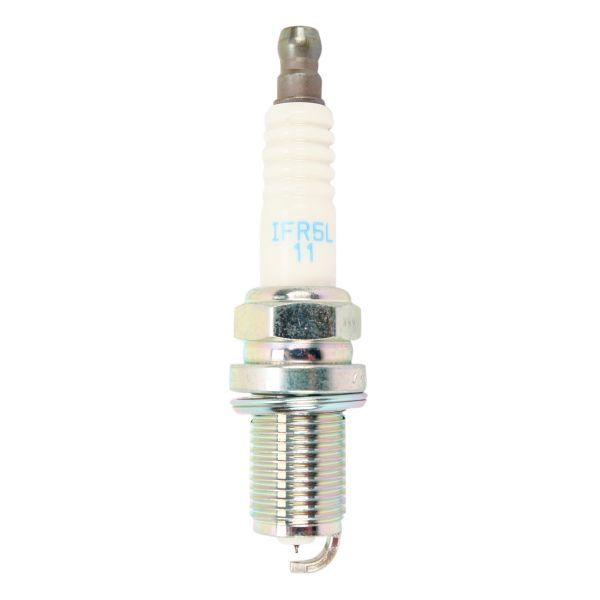
\includegraphics[width=0.4\textwidth]{reference/picture/bougie.jpg}
    \caption{IHM de l'application}
\end{figure}
\subsection{Présentation DA}
L'objectif de l'interface est de proposer les fonctionnalités de notre programme au travers d'une interfaces graphiques permettants de sélectionner les différentes méthodes de seuillage, le type de seuil, la tailles des patchs ainsi que la valeur du bruit. \par
Une autre fonctionnalité que nous voulions implémenter est l'affichage de l'image de départ, bruitée ainsi que le résultats final. Il est également important d'afficher les indicateurs de performances associés à la procédure que nous venons d'appliquer sur l'image. \par
Enfin, une action de débruitage optimal est implémenter dans l'IHM afin qu'un utilisateurs puissent, à partir d'une image bruité avoir le meilleur retour des 8 méthodes.
\subsection{Justification}
Pour le principe de l'IHM, nous avons voulu suivre les étapes suivantes :
\begin{enumerate}
    \item Charger une image localement
    \item Lui appliquer un bruitage en fonction d'une contante \(\sigma\) choisis par l'utilisateurs
    \item Choisir le type d'extraction, la taille des patchs, la méthode de seuillage et le type de seuil
    \item Lecture des indicateurs de performances
    \item Exporter les résultats
\end{enumerate}

Pour le choix du sigma, nous avons choisis un slider permettant facilement de sélectionner sigma dans un intervalle de valuer. Pour le reste des paramètres, nous avons utilisé des menus déroulants car les choix des possibilités est restreint. \par
Pour les actions de bruitage, débruitages sous paramètres et débruitage optimal, nous avons insérer 3 boutons correspondant à chacune de ces actions. \par
Enfin, nous avons la possibilité d'enregistrer, de réinitialiser,  au travers de deux boutons situés en bas de page